\documentclass{article}%
\usepackage[T1]{fontenc}%
\usepackage[utf8]{inputenc}%
\usepackage{lmodern}%
\usepackage{textcomp}%
\usepackage{lastpage}%
\usepackage[head=40pt,margin=0.5in,bottom=0.6in]{geometry}%
\usepackage{graphicx}%
%
\title{\textbf{Liberan a periodista Mario Peláez después de imputarlo por "instigación al orden público"}}%
\author{VALENTÍN ROMERO MARTÍNEZ}%
\date{03/03/2019}%
%
\begin{document}%
\normalsize%
\maketitle%
\textbf{URL: }%
http://www.eluniversal.com/politica/34708/liberan{-}a{-}periodista{-}mario{-}pelaez{-}despues{-}de{-}imputarlo{-}por{-}instigacion{-}al{-}orden{-}publico\newline%
%
\textbf{Periodico: }%
EU, %
ID: %
34708, %
Seccion: %
politica\newline%
%
\textbf{Palabras Claves: }%
NO\_TIENE\newline%
%
\textbf{Derecho: }%
2.1%
, Otros Derechos: %
\newline%
%
\textbf{\textit{El jefe de redacción del diario El Caribazo de Nueva Esparta tendrá que presentarse cada ocho días ante el tribunal de la causa junto a tres personas con las que fue detenido el pasado 27 de febrero}}%
\newline%
\newline%
%
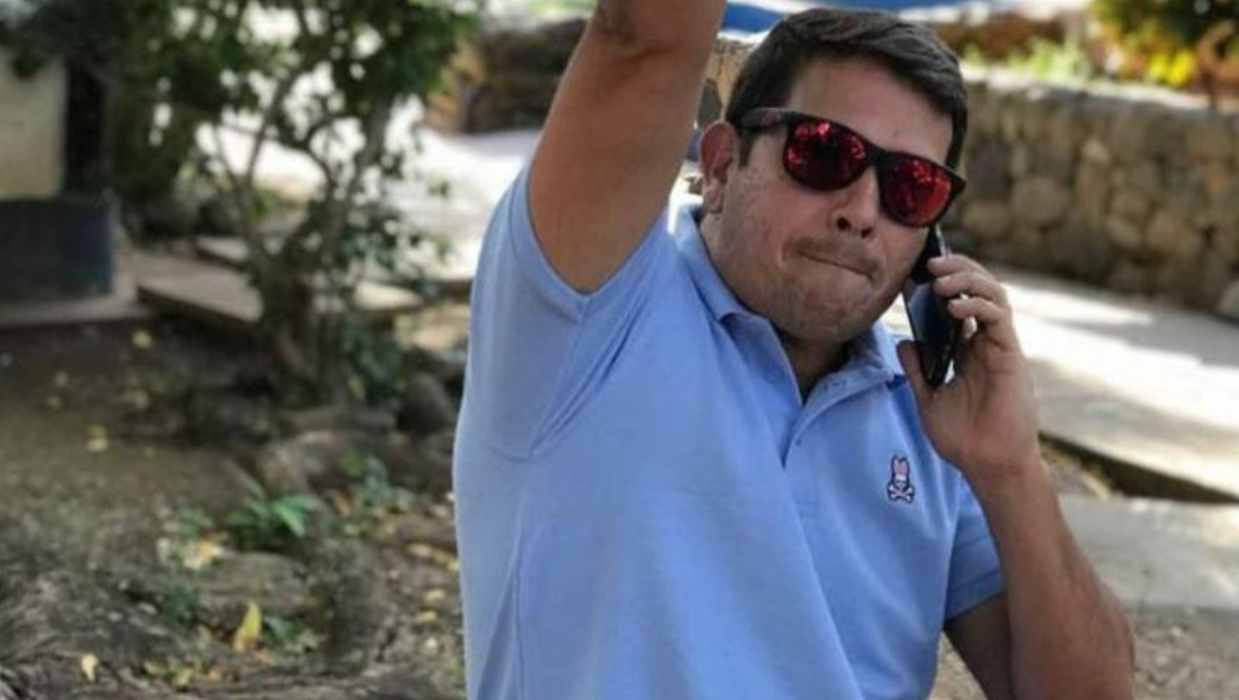
\includegraphics[width=300px]{EU_34708.jpg}%
\newline%
%
Caracas.{-} El periodista Mario Peláez, quien se encontraba detenido desde el pasado 27 de febrero, fue liberado este domingo con régimen de presentación cada ocho días, luego de ser imputado por "instigación al orden público".%
\newline%
%
La información fue suministrada por el Sindicato Nacional de Periodistas (SNTP) en su cuenta de Twitter, por donde había denunciado su detención y responsabilizaba al Gobierno por su integridad y la de sus acompañantes quienes fueron despojados de sus teléfonos celulares y fueron entregados al Sebin.%
\newline%
%
Junto al comunicador social fueron arrestados Juan Bautista Mata, Nilson Torres y Victor Cirios, cuando volvían de Colombia donde Peláez cubrió~el fallido ingreso de ayuda humanitaria del pasado 23 de febrero. A estos ciudadanos les dictaron la misma medida sustitutiva.%
\newline%
%
El SNTP también denunció que después de 72 horas detenido "fue presentado en un tribunal con competencia en delitos económicos" y la jueza había declinado la causa, siendo llevado después a "un tribunal contra el terrorismo", ante la misma jueza de la causa del diputado Juan Requesens.%
\newline%
%
"No hay nada en las actas que comprometa o vincule al periodista Mario Peláez con actos de terrorismo. Que sepa el mundo que Nicolás Maduro ensaya una nueva forma de acoso y silenciamiento contra la prensa", escribió el SNTP en la referida red social antes de que fuera dictada la sentencia.%
\newline%
%
\end{document}